\documentclass[a4paper, 11pt]{article}
\usepackage{amsmath}
\usepackage{amssymb}
\usepackage[T1]{fontenc}
\usepackage[utf8x]{inputenc}
\usepackage{lmodern}
\usepackage{graphicx}
\graphicspath{ {./images/} }
\usepackage[english]{babel} 
\usepackage{natbib}
\usepackage{cite}
\usepackage[parfill]{parskip}
\usepackage{enumerate}
\usepackage{float}%for image positions
\usepackage{hyperref}
\hypersetup{
    colorlinks,
    citecolor=black,
    filecolor=black,
    linkcolor=black,
    urlcolor=black
}
\usepackage{amsthm}
\newtheorem{theorem}{Theorem}[section]
\newtheorem{lemma}[theorem]{Lemma}
\newtheorem{proposition}[theorem]{Proposition}
\newtheorem{axiom}[theorem]{Axiom}
\newtheorem{invariant}[theorem]{Invariant}
\newtheorem{breakpoint}[theorem]{Breakpoint}
\newtheorem{problem}{Problem}
\newtheorem{definition}{Definition} 
\usepackage{algorithm}
\usepackage{algpseudocode}
\usepackage{pifont}
\usepackage{multirow,array}
\usepackage{centernot}
\usepackage{comment} % enables the use of multi-line comments (\ifx \fi) 
\usepackage{lipsum} %This package just generates Lorem Ipsum filler text. 
\usepackage{fullpage} % changes the margin

\begin{document}
\noindent
\large\textbf{Homework 1} \hfill \textbf{Kim Hammar} \\
\normalsize ID2209 \hfill Due Date: 14 November 2016 \\
Distributed Artifical Intelligence and Intelligent Agents \hfill \\

\section*{Problem Statement}
The given task was to implement a very basic MultiAgentSystem (M.A.S) in the JAVA Agent Development Framework (JADE) \citep{jade}, with the purpose of getting hands on experience with agent platforms and in particular the JADE agent platform. The assignment was also designed in a way to give experience programming agents in the context of a \textit{practical scenario}.

\section*{Main problems and solutions}
\begin{itemize}
\item \textit{Connecting agents through a platform that can be used for interaction and service discovery}

The JADE framework provides among other things a runtime environment, where JADE agents can ``live''. The agents in the M.A.S for this assignment are distributed on different JADE containers that all are connected to a single platform, which enable the agents to utilize the JADE runtime environment to find and interact with each other.

\item \textit{Agent design (micro perspective): designing agents that can act autonomously in a given environment and make decisions.}

Agents in this M.A.S perform tasks and perceive the environment to achieve their goals. Using JADE, the main mechanisms for designing and implementing agent tasks is through use of behaviours.
\item \textit{Society design (macro perspective): designing interactions for cooperation and coordination between agents in a M.A.S}

The Foundation for Intelligent Physical Agents (FIPA) is used as the main Agent Communication Language (ACL) between agents in this M.A.S.
\end{itemize}

\subsection*{Connecting Agents}
We refer to each running instance of JADE runtime environment as a Container, which can contain zero or more agents. The set of active containers is called a Platform and each platform have one container that is a special \textit{main container} \citep{jade_tutorial}. The most important aspect of the main container is to connect other containers together and to provide two important services: \textbf{AMS and DF}, AMS (Agent Management System) is a naming service that ensures that each agent in the platform has a unique name. DF (Directory Facilitator) aka ``The Yellow Pages'' is a service where agents can \textit{register} as providers of certain services and where agents can \textit{search} for providers of specific services. 

When running the M.A.S for this assignment the typical setup is to use $4$ containers:
\begin{enumerate}[I]
\item \textbf{Main container}: required container for connecting the other containers. Does not host any agents directly in this setup.
\item \textbf{Container 1}: Container where one ore more \textit{curator} agents live.
\item \textbf{Container 2}: Container where one ore more \textit{tourguide} agents live.
\item \textbf{Container 3}: Container where one ore more \textit{profiler} agents live.
\end{enumerate}
\subsection*{Agent Design}
There are three different types of agents in this system,
\begin{itemize}
\item \textbf{CuratorAgent}: Agent with the goal of monitoring an artgallery and respond to requests for art information from TourGuideAgents and ProfilerAgents. The CuratorAgent registers at the DF as a provider of the \texttt{artgallery-information} service, this agent perceives its environment mainly through the main container and its message-mailbox. The tasks/JADE behaviours of this agent are:
\begin{itemize}
\item A \texttt{ParallelBehaviour} consisting of three \texttt{SubBehaviours}:
\begin{itemize}
\item \texttt{GenreRequestServer} - A \texttt{CyclicBehaviour} that receives requests for a list of all genres of the monitored art gallery and responds to it.
\item \texttt{TourRequestServer} - A \texttt{CyclicBehaviour} that receives requests for a list of artifacts in the artgallery that matches a certain genre/interest and responds to it.
\item \texttt{ArtifactRequestServer} - A \texttt{CyclicBehaviour} that receives requests for details about a certain artifact in the artallery and responds to it.
\end{itemize}
\end{itemize}
\item \textbf{TourGuideAgent}: Agent with the goal to build virtual tours upon requests from ProfilerAgents. The TourGuideAgent interacts with CuratorAgents to retrieve information for tours. The TourGuideAgent registers at the DF as providing the \texttt{virtualtour} service, and perceives its environment mainly through the main container and its message-mailbox. The tasks/JADE behaviours of this agent are:
\begin{itemize}
\item A \texttt{ParallelBehaviour} consisting of three \texttt{SubBehaviours}:
\begin{itemize}
\item \texttt{CuratorSubscriber} - A \texttt{SubscriptionInitiator} behaviour that subscribes to the DF service to receive notifications when new agents that provide the \texttt{artgallery-information} service (a service that is provided by CuratorAgents) registers.
\item \texttt{ProfilerMatcher} - An \texttt{AchieveREResponder} that receives requests from ProfilerAgents asking what kind of genres it can build virtual tours for. This behaviour is linked to the \texttt{FindSupportedInterest} behaviour (which is an \texttt{AchieveREInitiator}) that will be invoked when a request is received in order to: \textit{(i)} ask discovered curator agents about their genres, \textit{(ii)} build a list of all genres, \textit{(iii)} respond to the requester with the list of genres.
\item \texttt{VirtualTourServer} - An \texttt{AchieveREResponder} that receives requests for virtual tours for specific interests/genres from profilers. When a request is received it will cause the \texttt{BuildVirtualTour} behaviour to be invoked which is an \texttt{AchieveREInitiator} that will send requests to all discovered curators and build a list of $\langle Artifact, Curator\rangle$ pairs that matches the given interest and finally it will respond with the built list to the requester.
\end{itemize}
\end{itemize}
\item \textbf{ProfilerAgent}: Agent that maintains the profile of a user and that has the goal of travelling around the network and collecting interesting (from the user's point of view) information about art. The agent perceives its environment mainly through the main container and input from the user. The tasks/JADE behaviours of this agent are:
\begin{itemize}
\item A \texttt{FSMBehaviour} consisting of $7$ states and $10$ different state transitions. The states are:
\begin{itemize}
\item \texttt{INITIALIZE\_USER\_PROFILE} - An \texttt{OneShotBehaviour} that interacts with the user for initializing the user profile (only invoked if command-line aguments were not supplied)
\item \texttt{SEARCH\_TOURGUIDES\_STATE} - An \texttt{OneShotBehaviour} that queries the DF for a list of all agents that provide the \texttt{virtualtour} service.
\item \texttt{FIND\_MATCHING\_TOUR\_GUIDES\_STATE} - An \texttt{AchieveREInitiator} that sends request-queries to all found TourGuideAgents asking what type of tours they provide.
\item \texttt{SELECT\_TOURGUIDE\_STATE} - An \texttt{OneShotBehaviour} for presenting the found tourguides and the types of tours they offer to the user and letting the user choose a tourguide.
\item \texttt{FIND\_VIRTUAL\_TOUR\_STATE} - An \texttt{AchieveREInitiator} that sends a request to a chosen tourguide, requesting a virtual tour matching the interest of the user.
\item \texttt{SELECT\_ARTIFACT\_STATE} - An \texttt{OneShotBehaviour} for presenting the virtual tour to the user and letting the user pick artifacts to visit.
\item \texttt{RETRIEVE\_ARTIFACT\_STATE} - An \texttt{AchieveREInitiator} that sends a request for details about the artifact to the curator of the artifact in the virtual tour that was selected. When the details are retrieved they are presented to the user.
\end{itemize}
\end{itemize}
\begin{figure}[H]
  \begin{center}
    \scalebox{0.90}{
      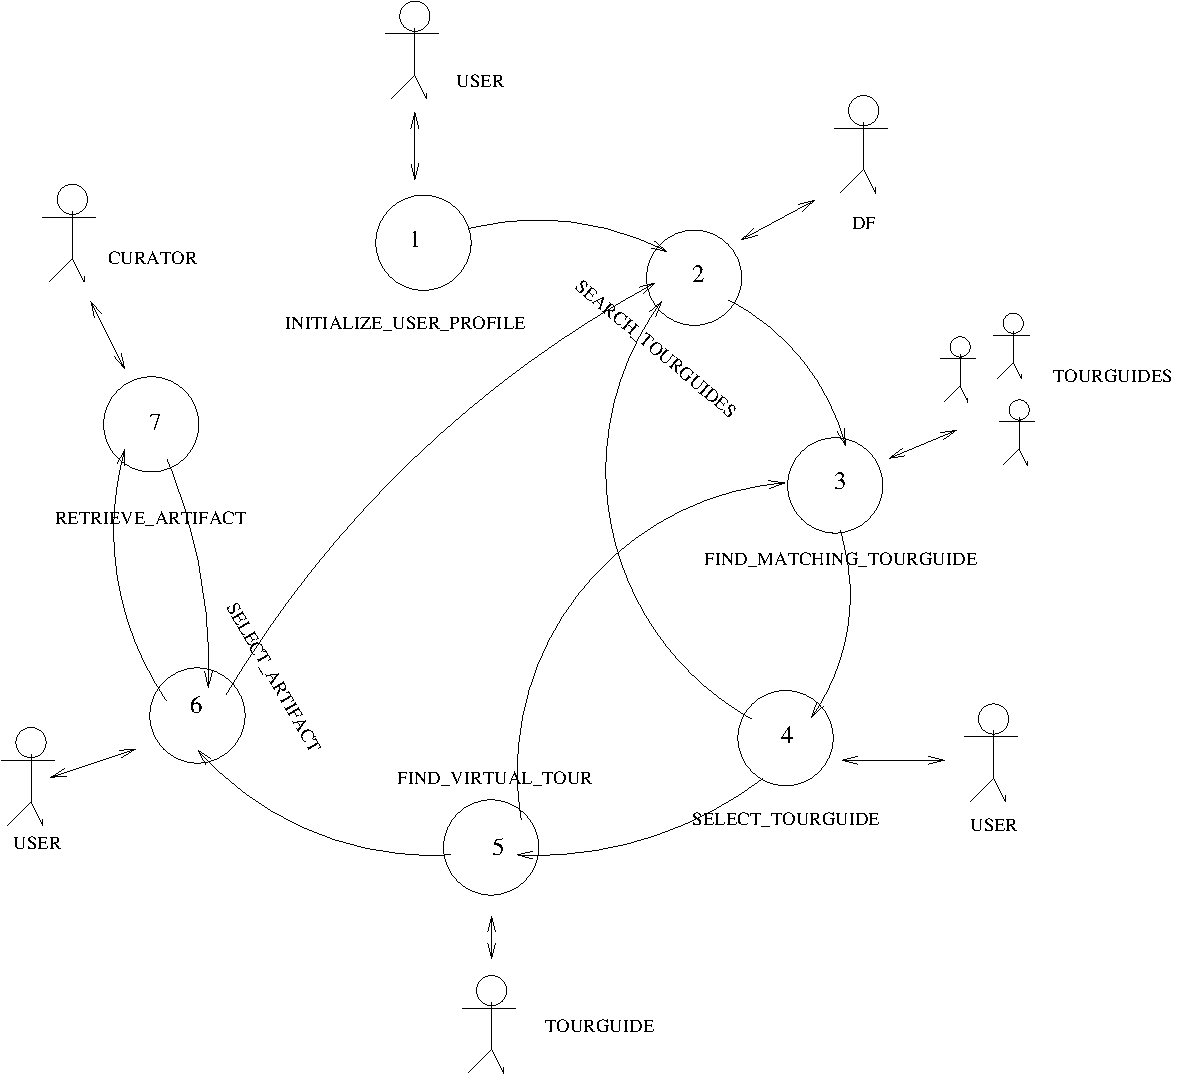
\includegraphics{fsm.pdf}
    }
    \caption{FSMBehaviour of ProfilerAgent}
    \label{fig:fsm}
  \end{center}
\end{figure}
\end{itemize}
\subsection*{Society Design}
From the presentation of the agent designs it should be clear that they need to interact in order to complete their individual goals. As mentioned, FIPA ACL is used for communication to gurarantee a consistent syntax of messages. The central concept for communication is that agents explicitly state a \textit{performative-verb} together with the content of each message. The performative verb decides how the agent at the receiving side will interpret the message. FIPA defines a large set of performative verbs, the main ones used in this M.A.S are:
\begin{description}
\item[query-ref] Used by one agent to determine the specific value for an expression \citep{coursebook}, for example when a profiler agent queries tour guides for the types of virtual tours they support.
\item[request] Allows an agent to request another agent to perform some action \citep{coursebook}, for example when a profiler agent requests a tourguide agent to build a virtual tour for a specific interest.
\item[agree] Used to indicate that the agent has agreed a request made by another agent \citep{coursebook}, for example when a tourguide receivs a request to build a virtual tour it responds with a message with this performative before actually building the tour.
\item[inform] Basic performative for communicating information \citep{coursebook}, used for example by an tourguide agent to inform a profiler \underline{after} having successfully built a virtual tour upon request.
\item[failure] Indicates that an attempt to perform some action failed \citep{coursebook}, used by tourguide agents to respond to profilers if they fail to build a virtual tour (for example if curators did not respond).
\end{description}
\section*{Conclusions}
Building a M.A.S consisting of autonomous agents that interact with each other is different to building ``regular'' distributed systems. In this assignment the agents were \textit{benevolent} towards each other which eased the development quite abit, since there were no need to be concerned about negotiations and agent-strategies. The main hurdle to overcome when developing this M.A.S as opposed to regular distributed systems was to understand how the agents interact through performative verbs, JADE libraries were useful in this aspect.

\section*{Attachments}
Documented source code can be found in the attached zipfile. See README.MD in the root directory for instruction on how to execute and build the program.

\bibliography{references}{}
\bibliographystyle{plain}
\end{document}